\documentclass[aspectratio=43,10pt]{beamer}

% ---------------------------------------------------------------- look & feel
\usetheme{Frankfurt}
\usepackage[T1]{fontenc}
\usepackage{lmodern}
\usepackage{amsmath,amssymb}
\usepackage{booktabs}
\usepackage{tikz}
\usetikzlibrary{arrows.meta,positioning,fit,calc,backgrounds}

\definecolor{tudnavy}{HTML}{0F2B46}
\definecolor{cNat}{HTML}{2A78D6}
\definecolor{cFsqF}{HTML}{EB6834}
\definecolor{cFsqJ}{HTML}{1BAF7A}
\definecolor{cJep}{HTML}{EDA100}
\definecolor{cGray}{HTML}{8A8A8A}

\setbeamercolor{structure}{fg=tudnavy}
\setbeamercolor{frametitle}{bg=tudnavy,fg=white}
\setbeamercolor{title}{bg=tudnavy,fg=white}
\setbeamercolor{section in head/foot}{bg=white,fg=tudnavy}
\setbeamercolor{subsection in head/foot}{bg=white,fg=tudnavy}
\setbeamercolor{footline}{bg=tudnavy,fg=white}
\setbeamercolor{item}{fg=tudnavy}
\setbeamercolor{block title}{bg=tudnavy,fg=white}
\setbeamercolor{block body}{bg=tudnavy!6}
\setbeamerfont{frametitle}{size=\large}
\setbeamertemplate{navigation symbols}{}
\setbeamertemplate{itemize items}[circle]
\setbeamertemplate{section in toc}[ball]
\setbeamertemplate{caption}[numbered]
\setbeamertemplate{frametitle}{%
  \nointerlineskip
  \begin{beamercolorbox}[wd=\paperwidth,ht=2.4ex,dp=1.1ex,leftskip=0.6em]{frametitle}
    \usebeamerfont{frametitle}\insertframetitle
  \end{beamercolorbox}}

% two-line footline as in the reference deck
\setbeamertemplate{footline}{%
  \leavevmode%
  \hbox{\begin{beamercolorbox}[wd=\paperwidth,ht=2.4ex,dp=0.9ex]{footline}%
    \scriptsize\hspace*{0.7em}\insertshortauthor\hfill\insertshortinstitute\hspace*{0.7em}%
  \end{beamercolorbox}}%
  \vskip0pt%
  \hbox{\begin{beamercolorbox}[wd=\paperwidth,ht=2.4ex,dp=1.1ex]{footline}%
    \scriptsize\hspace*{0.7em}\insertshorttitle\hfill\insertframenumber{} / \inserttotalframenumber\hspace*{0.7em}%
  \end{beamercolorbox}}}

% outline slide at the start of every section
\AtBeginSection[]{%
  \begin{frame}
    \vfill
    \tableofcontents[currentsection]
    \vfill
  \end{frame}}

\makeatletter\newcommand{\tabinput}[1]{\@@input #1 }\makeatother

% ---------------------------------------------------------------- title
\title[Universal Feature Extractor for Atari]{TOWARDS A UNIVERSAL FEATURE\\EXTRACTOR FOR ATARI GAMES}
\subtitle{Reconstruction, FSQ and Joint-Embedding Prediction}
\author{Sajid Ali Sadruddin}
\institute[Technische Universit\"at Dresden (TUD)]{Technische Universit\"at Dresden (TUD)}
\date{September, 2026}
\titlegraphic{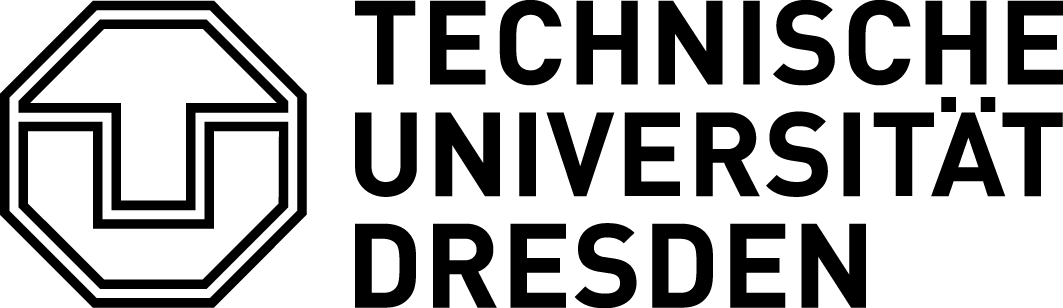
\includegraphics[width=3.2cm]{figures/tud_logo.png}}

\begin{document}

\begin{frame}
  \titlepage
\end{frame}

\begin{frame}
  \vfill
  \tableofcontents
  \vfill
\end{frame}

% =================================================================
\section{Introduction}

\begin{frame}{Introduction}
  \begin{itemize}\setlength\itemsep{0.6em}
    \item Atari games are one of the most common benchmarks for RL from pixels
    \item Every game gives the agent the same input: 4 stacked $84\times84$ grey-scale frames
    \item Still, each agent trains its own CNN feature extractor (NatureCNN) from scratch,
          using only the game reward
    \item Many games look alike: sprites, balls, walls and scrolling backgrounds
    \item \textbf{Idea:} pre-train \textbf{one} encoder on many games and reuse it for PPO
          on every game
  \end{itemize}
\end{frame}

\begin{frame}{Motivation and Research Questions}
  \begin{itemize}\setlength\itemsep{0.4em}
    \item A shared extractor could save training steps and compute, work on new games, and
          give one latent space for all games
    \item I looked at two design choices:
      \begin{itemize}
        \item \textbf{Objective:} reconstruct the pixels (VAE, VQ-VAE, FSQ-VAE) or predict the
              next state in latent space (V-JEPA)
        \item \textbf{Usage:} keep the encoder \emph{frozen} or \emph{fine-tune} it together
              with the policy
      \end{itemize}
  \end{itemize}
  \vspace{0.3em}
  \begin{block}{Research questions}
    \small
    \textbf{RQ1} Which objective gives the most useful features for PPO?\\
    \textbf{RQ2} Is it better to freeze or to fine-tune the encoder?\\
    \textbf{RQ3} Do the features work on games not seen in pre-training?\\
    \textbf{RQ4} What does it cost, and can we interpret the features?
  \end{block}
\end{frame}

% =================================================================
\section{Data \& Games}

\begin{frame}{Data Collection}
  \centering
  \resizebox{\textwidth}{!}{% Data collection and training-time processing, used as % Data collection and training-time processing, used as % Data collection and training-time processing, used as \input{figures/data_pipeline}
\resizebox{\textwidth}{!}{%
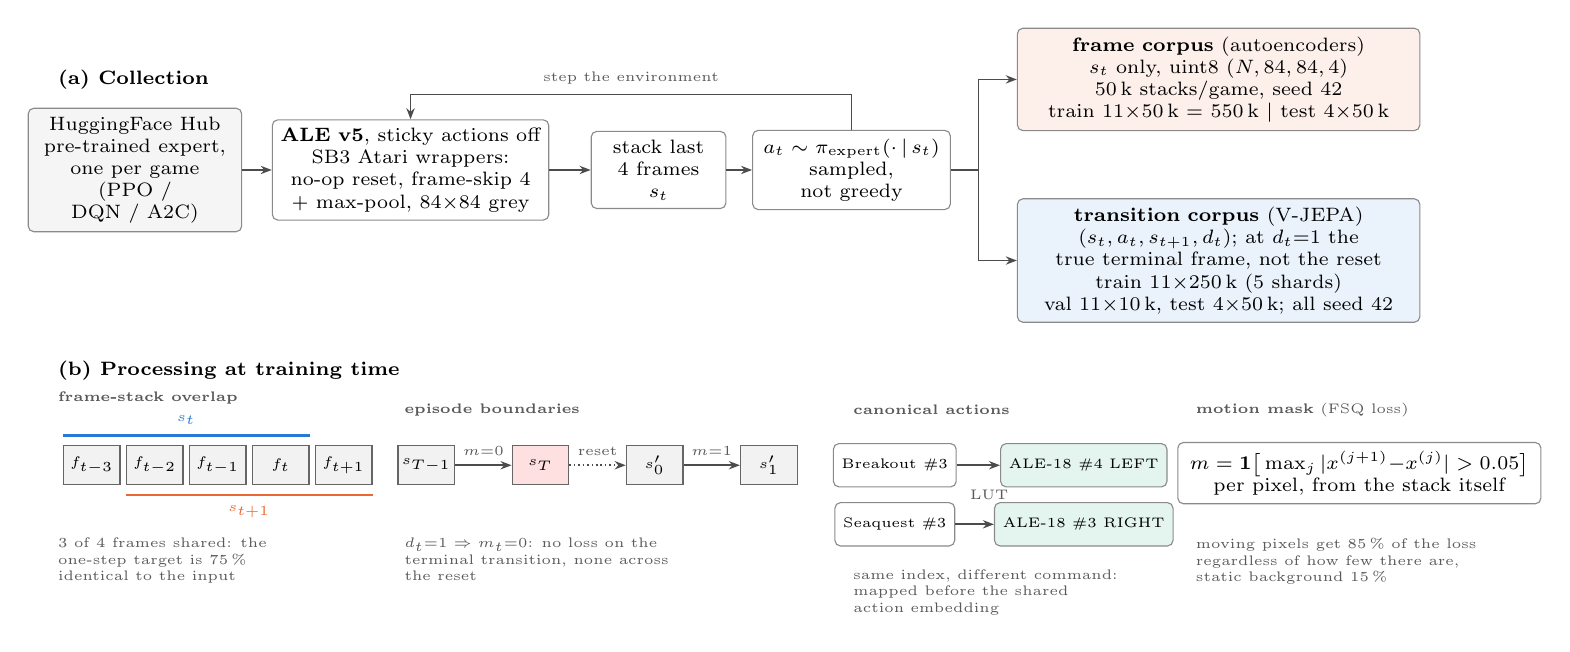
\begin{tikzpicture}[
  font=\scriptsize,
  box/.style={draw=cGray, rounded corners=2pt, align=center, inner sep=3pt, fill=white, minimum height=0.9cm},
  arr/.style={-{Stealth[length=4pt]}, draw=black!70, line width=0.6pt},
  fr/.style={draw=black!60, minimum width=0.72cm, minimum height=0.5cm, inner sep=0pt, font=\tiny},
  lab/.style={font=\tiny, text=black!65},
  ttl/.style={font=\scriptsize\bfseries, anchor=west}]

  % =========================================================== (a) collection
  \node[ttl] at (-1.1,3.35) {(a) Collection};
  \node[box, fill=gray!8, text width=2.5cm] (hub) at (0,2.2)
    {HuggingFace Hub\\pre-trained expert,\\one per game\\(PPO / DQN / A2C)};
  \node[box, text width=3.3cm] (env) at (3.5,2.2)
    {\textbf{ALE v5}, sticky actions off\\SB3 Atari wrappers: no-op reset, frame-skip 4 + max-pool, $84{\times}84$ grey};
  \node[box, text width=1.5cm] (stk) at (6.65,2.2) {stack last\\4 frames\\$s_t$};
  \node[box, text width=2.3cm] (pol) at (9.1,2.2) {$a_t\sim\pi_{\text{expert}}(\cdot\,|\,s_t)$\\sampled, not greedy};
  \draw[arr] (hub) -- (env); \draw[arr] (env) -- (stk); \draw[arr] (stk) -- (pol);
  \draw[arr] (pol.north) -- ++(0,0.45) -| node[pos=0.25, above, lab]{step the environment} (env.north);

  \node[box, fill=cFsqF!10, text width=4.9cm, anchor=west] (c1) at (11.2,3.35)
    {\textbf{frame corpus} (autoencoders)\\$s_t$ only, uint8 $(N,84,84,4)$\\50\,k stacks/game, seed 42\\train 11${\times}$50\,k = 550\,k $\mid$ test 4${\times}$50\,k};
  \node[box, fill=cNat!10, text width=4.9cm, anchor=west] (c2) at (11.2,1.05)
    {\textbf{transition corpus} (V-JEPA)\\$(s_t,a_t,s_{t+1},d_t)$; at $d_t{=}1$ the\\true terminal frame, not the reset\\train 11${\times}$250\,k (5 shards)\\val 11${\times}$10\,k, test 4${\times}$50\,k; all seed 42};
  \draw[arr] (pol.east) -- ++(0.35,0) |- (c1.west);
  \draw[arr] (pol.east) -- ++(0.35,0) |- (c2.west);

  % =========================================================== (b) processing
  \node[ttl] at (-1.1,-0.35) {(b) Processing at training time};

  % --- b1 frame overlap
  \node[lab, anchor=west] at (-1.1,-0.7) {\textbf{frame-stack overlap}};
  \foreach \i/\t in {0/$f_{t-3}$,1/$f_{t-2}$,2/$f_{t-1}$,3/$f_{t}$,4/$f_{t+1}$}
    {\node[fr, fill=gray!10] (f\i) at (-0.55+\i*0.8,-1.55) {\t};}
  \draw[cNat, line width=1pt] ([yshift=0.12cm]f0.north west) -- ([yshift=0.12cm]f3.north east)
     node[midway, above, font=\tiny, text=cNat] {$s_t$};
  \draw[cFsqF, line width=1pt] ([yshift=-0.12cm]f1.south west) -- ([yshift=-0.12cm]f4.south east)
     node[midway, below, font=\tiny, text=cFsqF] {$s_{t+1}$};
  \node[lab, align=left, anchor=north west] at (-1.1,-2.35) {3 of 4 frames shared: the\\one-step target is 75\,\%\\identical to the input};

  % --- b2 terminal mask
  \node[lab, anchor=west] at (3.3,-0.85) {\textbf{episode boundaries}};
  \node[fr, fill=gray!10] (e1) at (3.7,-1.55) {$s_{T-1}$};
  \node[fr, fill=red!12] (e2) at (5.15,-1.55) {$s_T$};
  \node[fr, fill=gray!10] (e3) at (6.6,-1.55) {$s'_0$};
  \node[fr, fill=gray!10] (e4) at (8.05,-1.55) {$s'_1$};
  \draw[arr] (e1) -- node[above, lab]{$m{=}0$} (e2);
  \draw[arr, densely dotted] (e2) -- node[above, lab]{reset} (e3);
  \draw[arr] (e3) -- node[above, lab]{$m{=}1$} (e4);
  \node[lab, align=left, anchor=north west] at (3.3,-2.35) {$d_t{=}1\Rightarrow m_t{=}0$: no loss on the\\terminal transition, none across\\the reset};

  % --- b3 action canonicalisation
  \node[lab, anchor=west] at (9.0,-0.85) {\textbf{canonical actions}};
  \node[box, minimum height=0.55cm, font=\tiny] (bk) at (9.65,-1.55) {Breakout \#3};
  \node[box, minimum height=0.55cm, font=\tiny] (sq) at (9.65,-2.3) {Seaquest \#3};
  \node[box, minimum height=0.55cm, font=\tiny, fill=cFsqJ!12] (l4) at (12.05,-1.55) {ALE-18 \#4 LEFT};
  \node[box, minimum height=0.55cm, font=\tiny, fill=cFsqJ!12] (r3) at (12.05,-2.3) {ALE-18 \#3 RIGHT};
  \draw[arr] (bk) -- (l4); \node[lab] at (10.85,-1.93) {LUT}; \draw[arr] (sq) -- (r3);
  \node[lab, align=left, anchor=north west] at (9.0,-2.75) {same index, different command:\\mapped before the shared\\action embedding};

  % --- b4 motion mask
  \node[lab, anchor=west] at (13.35,-0.85) {\textbf{motion mask} (FSQ loss)};
  \node[box, minimum height=0.55cm, text width=4.4cm, font=\scriptsize] (mm) at (15.55,-1.65)
    {\mbox{$m=\mathbf{1}\big[\max_j|x^{(j+1)}{-}x^{(j)}|>0.05\big]$}\\per pixel, from the stack itself};
  \node[lab, align=left, anchor=north west] at (13.35,-2.35) {moving pixels get 85\,\% of the loss\\regardless of how few there are,\\static background 15\,\%};
\end{tikzpicture}}

\resizebox{\textwidth}{!}{%
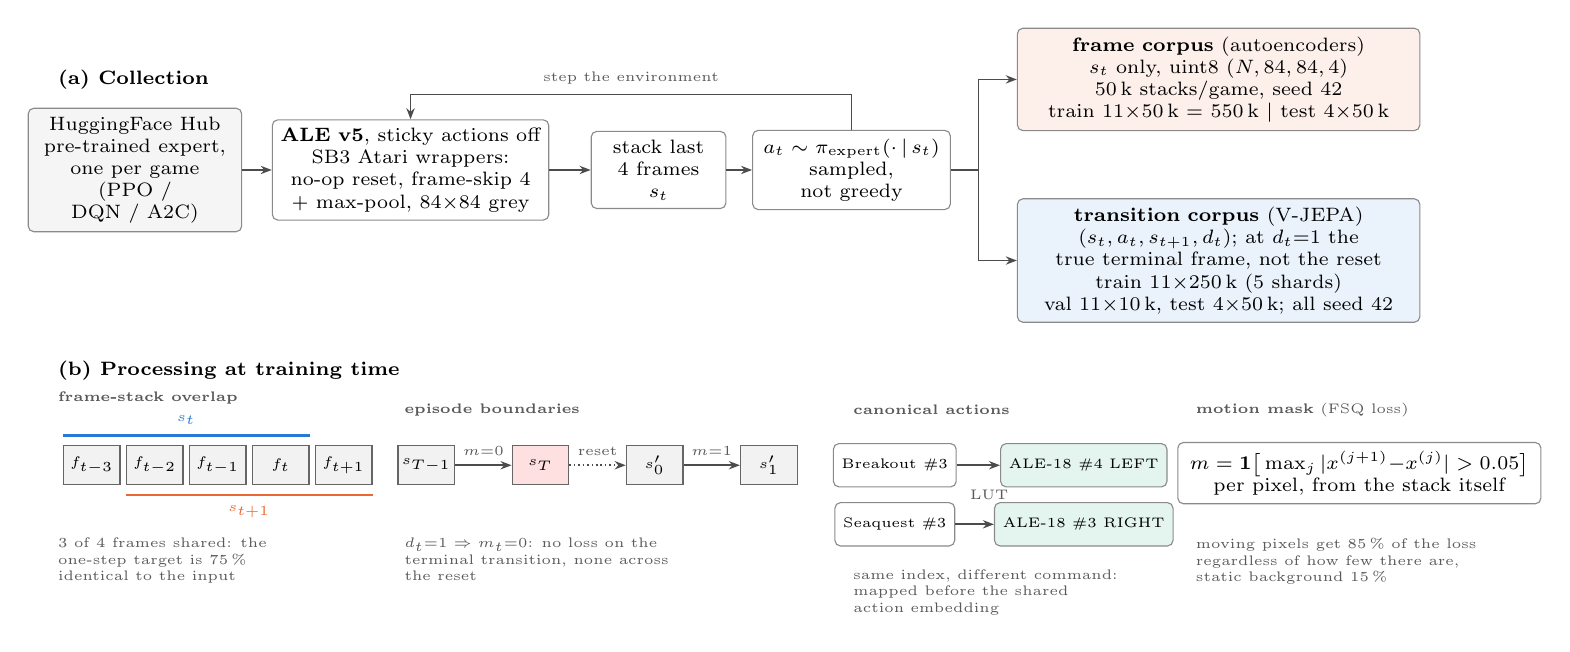
\begin{tikzpicture}[
  font=\scriptsize,
  box/.style={draw=cGray, rounded corners=2pt, align=center, inner sep=3pt, fill=white, minimum height=0.9cm},
  arr/.style={-{Stealth[length=4pt]}, draw=black!70, line width=0.6pt},
  fr/.style={draw=black!60, minimum width=0.72cm, minimum height=0.5cm, inner sep=0pt, font=\tiny},
  lab/.style={font=\tiny, text=black!65},
  ttl/.style={font=\scriptsize\bfseries, anchor=west}]

  % =========================================================== (a) collection
  \node[ttl] at (-1.1,3.35) {(a) Collection};
  \node[box, fill=gray!8, text width=2.5cm] (hub) at (0,2.2)
    {HuggingFace Hub\\pre-trained expert,\\one per game\\(PPO / DQN / A2C)};
  \node[box, text width=3.3cm] (env) at (3.5,2.2)
    {\textbf{ALE v5}, sticky actions off\\SB3 Atari wrappers: no-op reset, frame-skip 4 + max-pool, $84{\times}84$ grey};
  \node[box, text width=1.5cm] (stk) at (6.65,2.2) {stack last\\4 frames\\$s_t$};
  \node[box, text width=2.3cm] (pol) at (9.1,2.2) {$a_t\sim\pi_{\text{expert}}(\cdot\,|\,s_t)$\\sampled, not greedy};
  \draw[arr] (hub) -- (env); \draw[arr] (env) -- (stk); \draw[arr] (stk) -- (pol);
  \draw[arr] (pol.north) -- ++(0,0.45) -| node[pos=0.25, above, lab]{step the environment} (env.north);

  \node[box, fill=cFsqF!10, text width=4.9cm, anchor=west] (c1) at (11.2,3.35)
    {\textbf{frame corpus} (autoencoders)\\$s_t$ only, uint8 $(N,84,84,4)$\\50\,k stacks/game, seed 42\\train 11${\times}$50\,k = 550\,k $\mid$ test 4${\times}$50\,k};
  \node[box, fill=cNat!10, text width=4.9cm, anchor=west] (c2) at (11.2,1.05)
    {\textbf{transition corpus} (V-JEPA)\\$(s_t,a_t,s_{t+1},d_t)$; at $d_t{=}1$ the\\true terminal frame, not the reset\\train 11${\times}$250\,k (5 shards)\\val 11${\times}$10\,k, test 4${\times}$50\,k; all seed 42};
  \draw[arr] (pol.east) -- ++(0.35,0) |- (c1.west);
  \draw[arr] (pol.east) -- ++(0.35,0) |- (c2.west);

  % =========================================================== (b) processing
  \node[ttl] at (-1.1,-0.35) {(b) Processing at training time};

  % --- b1 frame overlap
  \node[lab, anchor=west] at (-1.1,-0.7) {\textbf{frame-stack overlap}};
  \foreach \i/\t in {0/$f_{t-3}$,1/$f_{t-2}$,2/$f_{t-1}$,3/$f_{t}$,4/$f_{t+1}$}
    {\node[fr, fill=gray!10] (f\i) at (-0.55+\i*0.8,-1.55) {\t};}
  \draw[cNat, line width=1pt] ([yshift=0.12cm]f0.north west) -- ([yshift=0.12cm]f3.north east)
     node[midway, above, font=\tiny, text=cNat] {$s_t$};
  \draw[cFsqF, line width=1pt] ([yshift=-0.12cm]f1.south west) -- ([yshift=-0.12cm]f4.south east)
     node[midway, below, font=\tiny, text=cFsqF] {$s_{t+1}$};
  \node[lab, align=left, anchor=north west] at (-1.1,-2.35) {3 of 4 frames shared: the\\one-step target is 75\,\%\\identical to the input};

  % --- b2 terminal mask
  \node[lab, anchor=west] at (3.3,-0.85) {\textbf{episode boundaries}};
  \node[fr, fill=gray!10] (e1) at (3.7,-1.55) {$s_{T-1}$};
  \node[fr, fill=red!12] (e2) at (5.15,-1.55) {$s_T$};
  \node[fr, fill=gray!10] (e3) at (6.6,-1.55) {$s'_0$};
  \node[fr, fill=gray!10] (e4) at (8.05,-1.55) {$s'_1$};
  \draw[arr] (e1) -- node[above, lab]{$m{=}0$} (e2);
  \draw[arr, densely dotted] (e2) -- node[above, lab]{reset} (e3);
  \draw[arr] (e3) -- node[above, lab]{$m{=}1$} (e4);
  \node[lab, align=left, anchor=north west] at (3.3,-2.35) {$d_t{=}1\Rightarrow m_t{=}0$: no loss on the\\terminal transition, none across\\the reset};

  % --- b3 action canonicalisation
  \node[lab, anchor=west] at (9.0,-0.85) {\textbf{canonical actions}};
  \node[box, minimum height=0.55cm, font=\tiny] (bk) at (9.65,-1.55) {Breakout \#3};
  \node[box, minimum height=0.55cm, font=\tiny] (sq) at (9.65,-2.3) {Seaquest \#3};
  \node[box, minimum height=0.55cm, font=\tiny, fill=cFsqJ!12] (l4) at (12.05,-1.55) {ALE-18 \#4 LEFT};
  \node[box, minimum height=0.55cm, font=\tiny, fill=cFsqJ!12] (r3) at (12.05,-2.3) {ALE-18 \#3 RIGHT};
  \draw[arr] (bk) -- (l4); \node[lab] at (10.85,-1.93) {LUT}; \draw[arr] (sq) -- (r3);
  \node[lab, align=left, anchor=north west] at (9.0,-2.75) {same index, different command:\\mapped before the shared\\action embedding};

  % --- b4 motion mask
  \node[lab, anchor=west] at (13.35,-0.85) {\textbf{motion mask} (FSQ loss)};
  \node[box, minimum height=0.55cm, text width=4.4cm, font=\scriptsize] (mm) at (15.55,-1.65)
    {\mbox{$m=\mathbf{1}\big[\max_j|x^{(j+1)}{-}x^{(j)}|>0.05\big]$}\\per pixel, from the stack itself};
  \node[lab, align=left, anchor=north west] at (13.35,-2.35) {moving pixels get 85\,\% of the loss\\regardless of how few there are,\\static background 15\,\%};
\end{tikzpicture}}

\resizebox{\textwidth}{!}{%
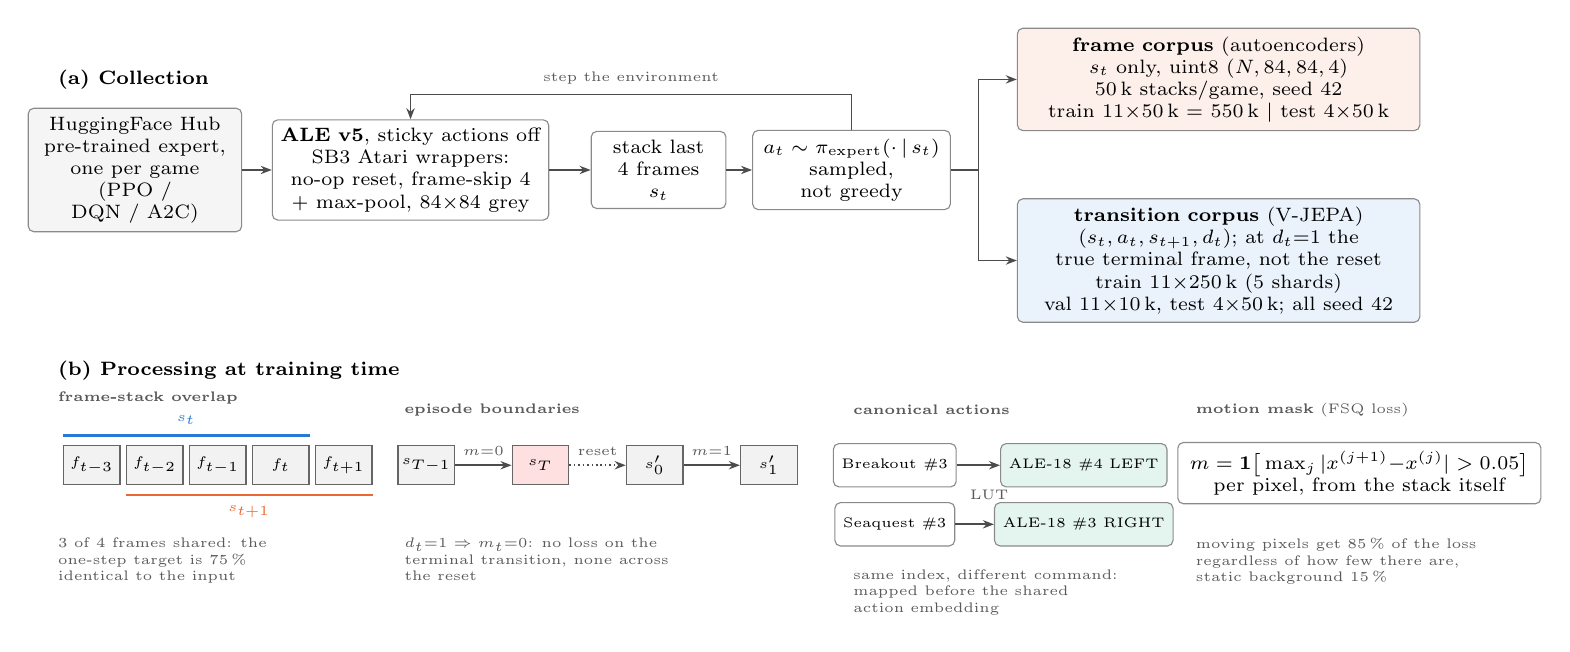
\begin{tikzpicture}[
  font=\scriptsize,
  box/.style={draw=cGray, rounded corners=2pt, align=center, inner sep=3pt, fill=white, minimum height=0.9cm},
  arr/.style={-{Stealth[length=4pt]}, draw=black!70, line width=0.6pt},
  fr/.style={draw=black!60, minimum width=0.72cm, minimum height=0.5cm, inner sep=0pt, font=\tiny},
  lab/.style={font=\tiny, text=black!65},
  ttl/.style={font=\scriptsize\bfseries, anchor=west}]

  % =========================================================== (a) collection
  \node[ttl] at (-1.1,3.35) {(a) Collection};
  \node[box, fill=gray!8, text width=2.5cm] (hub) at (0,2.2)
    {HuggingFace Hub\\pre-trained expert,\\one per game\\(PPO / DQN / A2C)};
  \node[box, text width=3.3cm] (env) at (3.5,2.2)
    {\textbf{ALE v5}, sticky actions off\\SB3 Atari wrappers: no-op reset, frame-skip 4 + max-pool, $84{\times}84$ grey};
  \node[box, text width=1.5cm] (stk) at (6.65,2.2) {stack last\\4 frames\\$s_t$};
  \node[box, text width=2.3cm] (pol) at (9.1,2.2) {$a_t\sim\pi_{\text{expert}}(\cdot\,|\,s_t)$\\sampled, not greedy};
  \draw[arr] (hub) -- (env); \draw[arr] (env) -- (stk); \draw[arr] (stk) -- (pol);
  \draw[arr] (pol.north) -- ++(0,0.45) -| node[pos=0.25, above, lab]{step the environment} (env.north);

  \node[box, fill=cFsqF!10, text width=4.9cm, anchor=west] (c1) at (11.2,3.35)
    {\textbf{frame corpus} (autoencoders)\\$s_t$ only, uint8 $(N,84,84,4)$\\50\,k stacks/game, seed 42\\train 11${\times}$50\,k = 550\,k $\mid$ test 4${\times}$50\,k};
  \node[box, fill=cNat!10, text width=4.9cm, anchor=west] (c2) at (11.2,1.05)
    {\textbf{transition corpus} (V-JEPA)\\$(s_t,a_t,s_{t+1},d_t)$; at $d_t{=}1$ the\\true terminal frame, not the reset\\train 11${\times}$250\,k (5 shards)\\val 11${\times}$10\,k, test 4${\times}$50\,k; all seed 42};
  \draw[arr] (pol.east) -- ++(0.35,0) |- (c1.west);
  \draw[arr] (pol.east) -- ++(0.35,0) |- (c2.west);

  % =========================================================== (b) processing
  \node[ttl] at (-1.1,-0.35) {(b) Processing at training time};

  % --- b1 frame overlap
  \node[lab, anchor=west] at (-1.1,-0.7) {\textbf{frame-stack overlap}};
  \foreach \i/\t in {0/$f_{t-3}$,1/$f_{t-2}$,2/$f_{t-1}$,3/$f_{t}$,4/$f_{t+1}$}
    {\node[fr, fill=gray!10] (f\i) at (-0.55+\i*0.8,-1.55) {\t};}
  \draw[cNat, line width=1pt] ([yshift=0.12cm]f0.north west) -- ([yshift=0.12cm]f3.north east)
     node[midway, above, font=\tiny, text=cNat] {$s_t$};
  \draw[cFsqF, line width=1pt] ([yshift=-0.12cm]f1.south west) -- ([yshift=-0.12cm]f4.south east)
     node[midway, below, font=\tiny, text=cFsqF] {$s_{t+1}$};
  \node[lab, align=left, anchor=north west] at (-1.1,-2.35) {3 of 4 frames shared: the\\one-step target is 75\,\%\\identical to the input};

  % --- b2 terminal mask
  \node[lab, anchor=west] at (3.3,-0.85) {\textbf{episode boundaries}};
  \node[fr, fill=gray!10] (e1) at (3.7,-1.55) {$s_{T-1}$};
  \node[fr, fill=red!12] (e2) at (5.15,-1.55) {$s_T$};
  \node[fr, fill=gray!10] (e3) at (6.6,-1.55) {$s'_0$};
  \node[fr, fill=gray!10] (e4) at (8.05,-1.55) {$s'_1$};
  \draw[arr] (e1) -- node[above, lab]{$m{=}0$} (e2);
  \draw[arr, densely dotted] (e2) -- node[above, lab]{reset} (e3);
  \draw[arr] (e3) -- node[above, lab]{$m{=}1$} (e4);
  \node[lab, align=left, anchor=north west] at (3.3,-2.35) {$d_t{=}1\Rightarrow m_t{=}0$: no loss on the\\terminal transition, none across\\the reset};

  % --- b3 action canonicalisation
  \node[lab, anchor=west] at (9.0,-0.85) {\textbf{canonical actions}};
  \node[box, minimum height=0.55cm, font=\tiny] (bk) at (9.65,-1.55) {Breakout \#3};
  \node[box, minimum height=0.55cm, font=\tiny] (sq) at (9.65,-2.3) {Seaquest \#3};
  \node[box, minimum height=0.55cm, font=\tiny, fill=cFsqJ!12] (l4) at (12.05,-1.55) {ALE-18 \#4 LEFT};
  \node[box, minimum height=0.55cm, font=\tiny, fill=cFsqJ!12] (r3) at (12.05,-2.3) {ALE-18 \#3 RIGHT};
  \draw[arr] (bk) -- (l4); \node[lab] at (10.85,-1.93) {LUT}; \draw[arr] (sq) -- (r3);
  \node[lab, align=left, anchor=north west] at (9.0,-2.75) {same index, different command:\\mapped before the shared\\action embedding};

  % --- b4 motion mask
  \node[lab, anchor=west] at (13.35,-0.85) {\textbf{motion mask} (FSQ loss)};
  \node[box, minimum height=0.55cm, text width=4.4cm, font=\scriptsize] (mm) at (15.55,-1.65)
    {\mbox{$m=\mathbf{1}\big[\max_j|x^{(j+1)}{-}x^{(j)}|>0.05\big]$}\\per pixel, from the stack itself};
  \node[lab, align=left, anchor=north west] at (13.35,-2.35) {moving pixels get 85\,\% of the loss\\regardless of how few there are,\\static background 15\,\%};
\end{tikzpicture}}
}
  \vspace{0.4em}
  \begin{itemize}\small
    \item Random play rarely leaves the first screen, so I used expert agents from HuggingFace
          (actions sampled, so some play is sub-optimal)
    \item \textbf{Frame dataset:} 50\,k frame stacks per game, for the autoencoders
    \item \textbf{Transition dataset:} 2.75\,M $(s_t,a_t,s_{t+1},d_t)$ from 11 games, for the V-JEPA
    \item 11 games for pre-training, 4 games held out for testing
  \end{itemize}
\end{frame}

\begin{frame}{The Games}
  \centering
  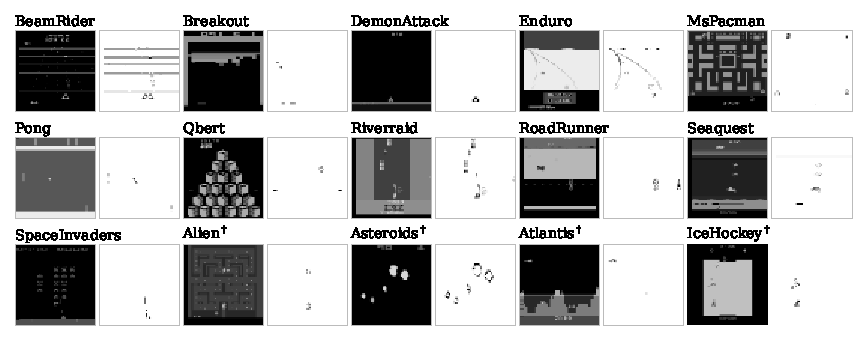
\includegraphics[width=\textwidth]{figures/games_grid.pdf}\\[0.3em]
  {\footnotesize Frame $t$ (left) and the change to the next frame (right) for all 15 games;
  $^\dagger$\,held-out games}
\end{frame}

\begin{frame}{How Different the Games Are}
  \begin{itemize}\setlength\itemsep{0.55em}
    \item \textbf{Appearance:} mean brightness goes from 5 (DemonAttack) to 105 (Pong), and
          1\% to 95\% of the pixels are black
    \item \textbf{Motion:} in most games less than 4\% of the pixels move (Pong 1.7\%,
          Breakout 1.4\%)
      \begin{itemize}
        \item The objects that matter for playing are a few small sprites
      \end{itemize}
    \item \textbf{Actions:} 4 to 18 actions per game, and the same index means a different
          button in different games
      \begin{itemize}
        \item For the V-JEPA, I mapped all games to one common set of 18 ALE actions
      \end{itemize}
    \item \textbf{Episodes:} from about 120 steps (Atlantis) to 12\,500 steps (Enduro)
    \item \textbf{Expert data:} the favourite action makes up 67\% of the steps in RoadRunner
          and 99\% in Asteroids, so there are few examples of other actions
  \end{itemize}
\end{frame}

% =================================================================
\section{Models}

\begin{frame}{Autoencoders}
  \begin{itemize}\setlength\itemsep{0.5em}
    \item \textbf{VAE:} NatureCNN encoder with a 256-dim latent vector, but its $7\times7$
          feature map is too coarse for small sprites (one cell = $12\times12$ pixels)
    \item \textbf{Residual VQ-VAE:} finer $21\times21$ grid, each cell replaced by one of
          $K=512$ codebook vectors
      \begin{itemize}
        \item Small moving objects went missing, so I trained a version where moving pixels
              count $10\times$
      \end{itemize}
    \item \textbf{FSQ-VAE:} each of 4 channels is simply rounded to $L=[8,5,5,3]$ levels
      \begin{itemize}
        \item No codebook to learn, so no unused codes
        \item New decoder (upsampling + conv) to remove checkerboard patterns
        \item Loss that gives moving pixels 85\% of the weight:
      \end{itemize}
  \end{itemize}
  \[
    \mathcal{L}_{\text{bal}} = 0.85\,\tfrac{\sum m\odot(\hat x-x)^2}{\sum m}
    +0.15\,\tfrac{\sum (1-m)\odot(\hat x-x)^2}{\sum (1-m)}
  \]
  \begin{itemize}
    \item Feature for PPO: the flattened $4\times21\times21$ grid (1\,764 values)
  \end{itemize}
\end{frame}

\begin{frame}{V-JEPA: Architecture}
  \centering
  \resizebox{\textwidth}{!}{% V-JEPA v2 architecture (atari-DQN-v2/JEPA.py), used as % V-JEPA v2 architecture (atari-DQN-v2/JEPA.py), used as % V-JEPA v2 architecture (atari-DQN-v2/JEPA.py), used as \input{figures/jepa_arch}
\resizebox{\textwidth}{!}{%
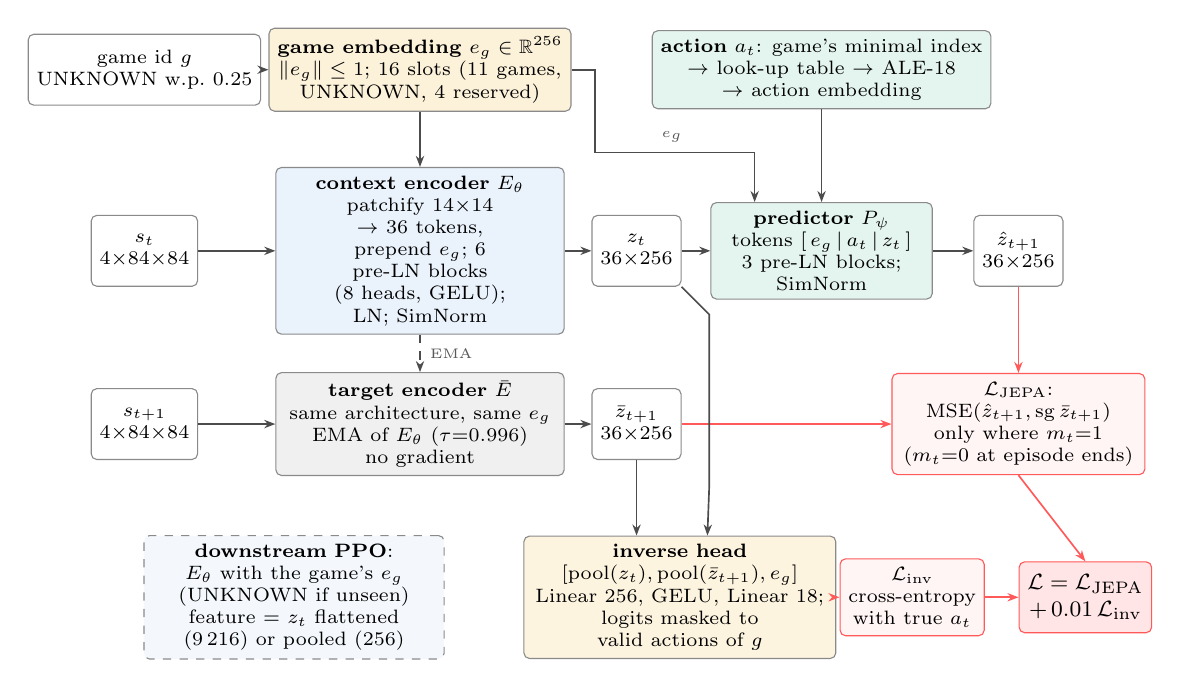
\begin{tikzpicture}[
  font=\scriptsize,
  box/.style={draw=cGray, rounded corners=2pt, align=center, inner sep=3pt, fill=white,
              minimum height=0.9cm},
  arr/.style={-{Stealth[length=4pt]}, draw=black!70, line width=0.6pt},
  larr/.style={-{Stealth[length=4pt]}, draw=red!65, line width=0.6pt},
  lab/.style={font=\tiny, text=black!65}]

  % ---------------------------------------------------------------- conditioning (top row)
  \node[box] (drop) at (0,4.5) {game id $g$\\UNKNOWN w.p.\ 0.25};
  \node[box, fill=cJep!15] (env) at (3.5,4.5)
    {\textbf{game embedding} $e_g\in\mathbb{R}^{256}$\\$\|e_g\|\le1$; 16 slots (11 games,\\UNKNOWN, 4 reserved)};
  \node[box, fill=cFsqJ!12] (act) at (8.6,4.5)
    {\textbf{action} $a_t$: game's minimal index\\$\to$ look-up table $\to$ ALE-18\\$\to$ action embedding};
  \draw[arr] (drop) -- (env);

  % ---------------------------------------------------------------- online branch
  \node[box] (st) at (0,2.2) {$s_t$\\$4{\times}84{\times}84$};
  \node[box, fill=cNat!10, text width=3.45cm] (ce) at (3.5,2.2)
    {\textbf{context encoder} $E_\theta$\\patchify $14{\times}14$ $\to$ 36 tokens,\\prepend $e_g$; 6 pre-LN blocks\\(8 heads, GELU); LN; SimNorm};
  \node[box] (zt) at (6.25,2.2) {$z_t$\\$36{\times}256$};
  \node[box, fill=cFsqJ!12, text width=2.6cm] (pr) at (8.6,2.2)
    {\textbf{predictor} $P_\psi$\\tokens $[\,e_g\,|\,a_t\,|\,z_t\,]$\\3 pre-LN blocks; SimNorm};
  \node[box] (zh) at (11.1,2.2) {$\hat z_{t+1}$\\$36{\times}256$};
  \draw[arr] (st) -- (ce); \draw[arr] (ce) -- (zt); \draw[arr] (zt) -- (pr); \draw[arr] (pr) -- (zh);
  \draw[arr] (env) -- (ce);
  \draw[arr] (act) -- (pr);
  \coordinate (ebend) at (7.75,3.45);
  \draw[arr] (env.east) -- ++(0.3,0) |- (ebend) -- (ebend |- pr.north);
  \node[lab, above] at (6.7,3.45) {$e_g$};

  % ---------------------------------------------------------------- target branch
  \node[box] (sn) at (0,0) {$s_{t+1}$\\$4{\times}84{\times}84$};
  \node[box, fill=gray!12, text width=3.45cm] (te) at (3.5,0)
    {\textbf{target encoder} $\bar E$\\same architecture, same $e_g$\\EMA of $E_\theta$ ($\tau{=}0.996$)\\no gradient};
  \node[box] (zb) at (6.25,0) {$\bar z_{t+1}$\\$36{\times}256$};
  \draw[arr] (sn) -- (te); \draw[arr] (te) -- (zb);
  \draw[arr, dashed] (ce) -- node[right, lab]{EMA} (te);

  % ---------------------------------------------------------------- losses
  \node[box, draw=red!65, fill=red!4, text width=3.0cm] (lj) at (11.1,0)
    {$\mathcal{L}_{\text{JEPA}}$: MSE$(\hat z_{t+1},\operatorname{sg}\bar z_{t+1})$\\only where $m_t{=}1$\\($m_t{=}0$ at episode ends)};
  \draw[larr] (zh) -- (lj);
  \draw[larr] (zb) -- (lj);

  \node[box, fill=cJep!12, text width=3.75cm] (inv) at (6.8,-2.2)
    {\textbf{inverse head}\\$[\operatorname{pool}(z_t),\operatorname{pool}(\bar z_{t+1}),e_g]$\\Linear 256, GELU, Linear 18;\\logits masked to valid actions of $g$};
  \draw[arr] (zt.south east) -- ++(0.35,-0.35) -- ++(0,-2.2) -- ([xshift=0.35cm]inv.north);
  \draw[arr] (zb) -- (zb |- inv.north);
  \node[box, draw=red!65, fill=red!4] (li) at (9.75,-2.2) {$\mathcal{L}_{\text{inv}}$\\cross-entropy\\with true $a_t$};
  \draw[larr] (inv) -- (li);
  \node[box, draw=red!65, fill=red!10, font=\footnotesize] (tot) at (11.95,-2.2)
    {$\mathcal{L}=\mathcal{L}_{\text{JEPA}}$\\$+\,0.01\,\mathcal{L}_{\text{inv}}$};
  \draw[larr] (li) -- (tot);
  \draw[larr] (lj.south) -- (tot.north);

  % ---------------------------------------------------------------- use in PPO
  \node[box, dashed, fill=cNat!5, text width=3.6cm] (ppo) at (1.9,-2.2)
    {\textbf{downstream PPO}: $E_\theta$ with the game's $e_g$ (UNKNOWN if unseen)\\feature = $z_t$ flattened (9\,216) or pooled (256)};
\end{tikzpicture}}

\resizebox{\textwidth}{!}{%
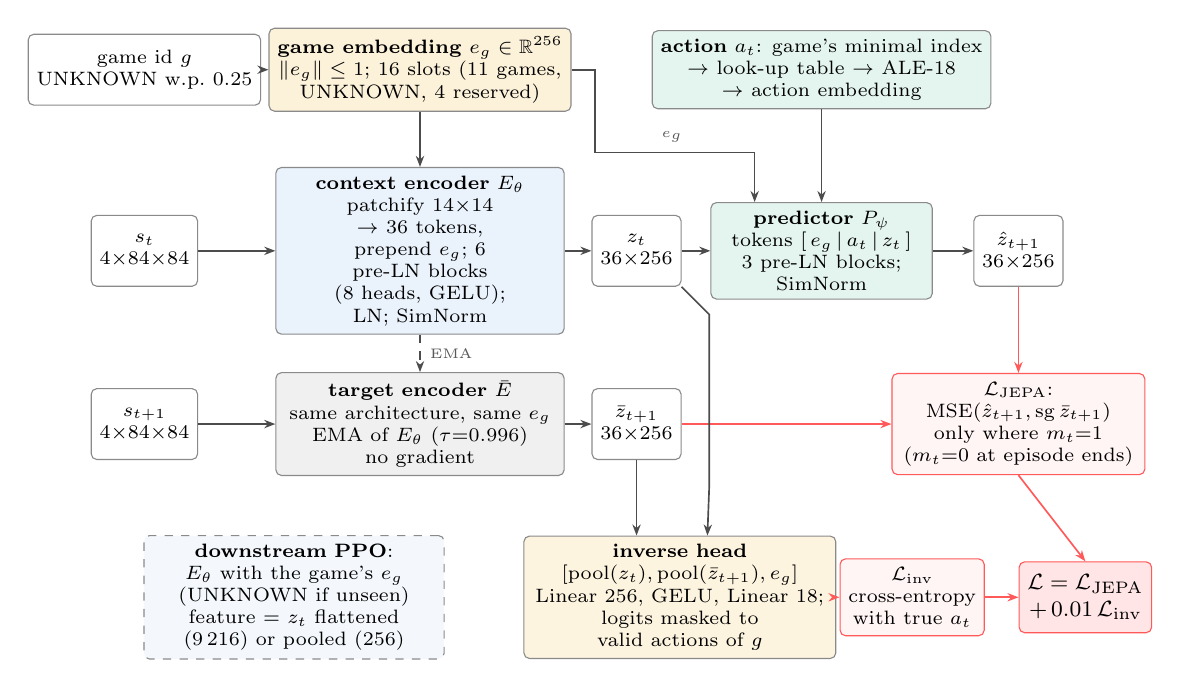
\begin{tikzpicture}[
  font=\scriptsize,
  box/.style={draw=cGray, rounded corners=2pt, align=center, inner sep=3pt, fill=white,
              minimum height=0.9cm},
  arr/.style={-{Stealth[length=4pt]}, draw=black!70, line width=0.6pt},
  larr/.style={-{Stealth[length=4pt]}, draw=red!65, line width=0.6pt},
  lab/.style={font=\tiny, text=black!65}]

  % ---------------------------------------------------------------- conditioning (top row)
  \node[box] (drop) at (0,4.5) {game id $g$\\UNKNOWN w.p.\ 0.25};
  \node[box, fill=cJep!15] (env) at (3.5,4.5)
    {\textbf{game embedding} $e_g\in\mathbb{R}^{256}$\\$\|e_g\|\le1$; 16 slots (11 games,\\UNKNOWN, 4 reserved)};
  \node[box, fill=cFsqJ!12] (act) at (8.6,4.5)
    {\textbf{action} $a_t$: game's minimal index\\$\to$ look-up table $\to$ ALE-18\\$\to$ action embedding};
  \draw[arr] (drop) -- (env);

  % ---------------------------------------------------------------- online branch
  \node[box] (st) at (0,2.2) {$s_t$\\$4{\times}84{\times}84$};
  \node[box, fill=cNat!10, text width=3.45cm] (ce) at (3.5,2.2)
    {\textbf{context encoder} $E_\theta$\\patchify $14{\times}14$ $\to$ 36 tokens,\\prepend $e_g$; 6 pre-LN blocks\\(8 heads, GELU); LN; SimNorm};
  \node[box] (zt) at (6.25,2.2) {$z_t$\\$36{\times}256$};
  \node[box, fill=cFsqJ!12, text width=2.6cm] (pr) at (8.6,2.2)
    {\textbf{predictor} $P_\psi$\\tokens $[\,e_g\,|\,a_t\,|\,z_t\,]$\\3 pre-LN blocks; SimNorm};
  \node[box] (zh) at (11.1,2.2) {$\hat z_{t+1}$\\$36{\times}256$};
  \draw[arr] (st) -- (ce); \draw[arr] (ce) -- (zt); \draw[arr] (zt) -- (pr); \draw[arr] (pr) -- (zh);
  \draw[arr] (env) -- (ce);
  \draw[arr] (act) -- (pr);
  \coordinate (ebend) at (7.75,3.45);
  \draw[arr] (env.east) -- ++(0.3,0) |- (ebend) -- (ebend |- pr.north);
  \node[lab, above] at (6.7,3.45) {$e_g$};

  % ---------------------------------------------------------------- target branch
  \node[box] (sn) at (0,0) {$s_{t+1}$\\$4{\times}84{\times}84$};
  \node[box, fill=gray!12, text width=3.45cm] (te) at (3.5,0)
    {\textbf{target encoder} $\bar E$\\same architecture, same $e_g$\\EMA of $E_\theta$ ($\tau{=}0.996$)\\no gradient};
  \node[box] (zb) at (6.25,0) {$\bar z_{t+1}$\\$36{\times}256$};
  \draw[arr] (sn) -- (te); \draw[arr] (te) -- (zb);
  \draw[arr, dashed] (ce) -- node[right, lab]{EMA} (te);

  % ---------------------------------------------------------------- losses
  \node[box, draw=red!65, fill=red!4, text width=3.0cm] (lj) at (11.1,0)
    {$\mathcal{L}_{\text{JEPA}}$: MSE$(\hat z_{t+1},\operatorname{sg}\bar z_{t+1})$\\only where $m_t{=}1$\\($m_t{=}0$ at episode ends)};
  \draw[larr] (zh) -- (lj);
  \draw[larr] (zb) -- (lj);

  \node[box, fill=cJep!12, text width=3.75cm] (inv) at (6.8,-2.2)
    {\textbf{inverse head}\\$[\operatorname{pool}(z_t),\operatorname{pool}(\bar z_{t+1}),e_g]$\\Linear 256, GELU, Linear 18;\\logits masked to valid actions of $g$};
  \draw[arr] (zt.south east) -- ++(0.35,-0.35) -- ++(0,-2.2) -- ([xshift=0.35cm]inv.north);
  \draw[arr] (zb) -- (zb |- inv.north);
  \node[box, draw=red!65, fill=red!4] (li) at (9.75,-2.2) {$\mathcal{L}_{\text{inv}}$\\cross-entropy\\with true $a_t$};
  \draw[larr] (inv) -- (li);
  \node[box, draw=red!65, fill=red!10, font=\footnotesize] (tot) at (11.95,-2.2)
    {$\mathcal{L}=\mathcal{L}_{\text{JEPA}}$\\$+\,0.01\,\mathcal{L}_{\text{inv}}$};
  \draw[larr] (li) -- (tot);
  \draw[larr] (lj.south) -- (tot.north);

  % ---------------------------------------------------------------- use in PPO
  \node[box, dashed, fill=cNat!5, text width=3.6cm] (ppo) at (1.9,-2.2)
    {\textbf{downstream PPO}: $E_\theta$ with the game's $e_g$ (UNKNOWN if unseen)\\feature = $z_t$ flattened (9\,216) or pooled (256)};
\end{tikzpicture}}

\resizebox{\textwidth}{!}{%
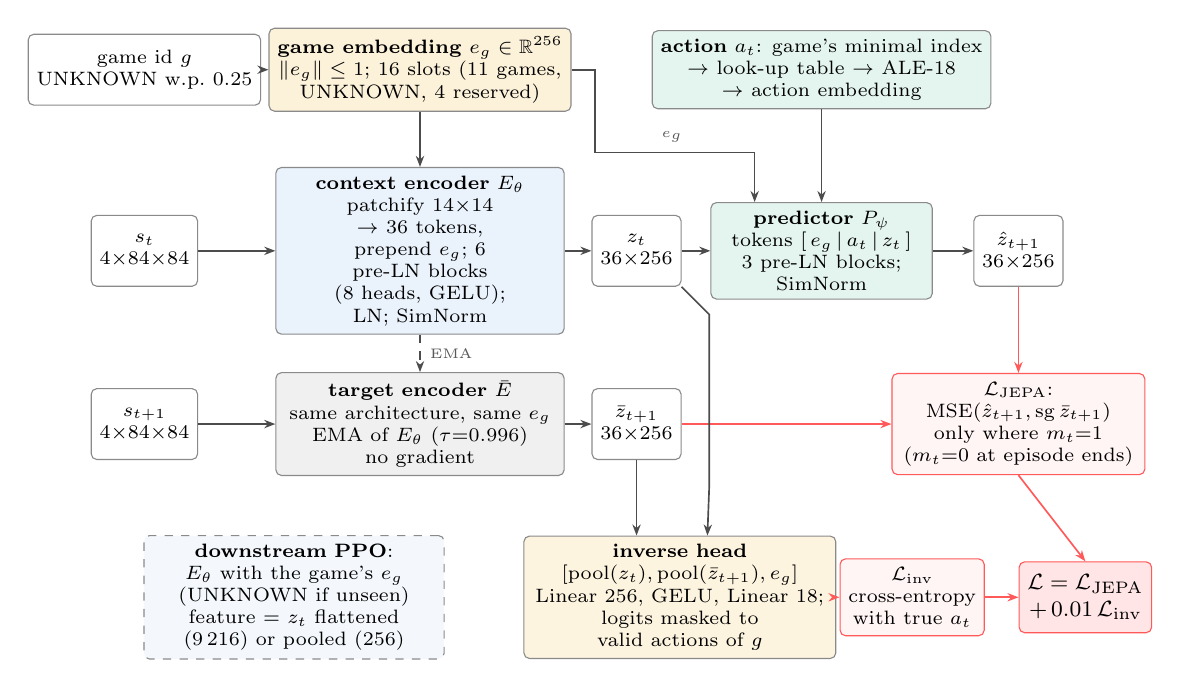
\begin{tikzpicture}[
  font=\scriptsize,
  box/.style={draw=cGray, rounded corners=2pt, align=center, inner sep=3pt, fill=white,
              minimum height=0.9cm},
  arr/.style={-{Stealth[length=4pt]}, draw=black!70, line width=0.6pt},
  larr/.style={-{Stealth[length=4pt]}, draw=red!65, line width=0.6pt},
  lab/.style={font=\tiny, text=black!65}]

  % ---------------------------------------------------------------- conditioning (top row)
  \node[box] (drop) at (0,4.5) {game id $g$\\UNKNOWN w.p.\ 0.25};
  \node[box, fill=cJep!15] (env) at (3.5,4.5)
    {\textbf{game embedding} $e_g\in\mathbb{R}^{256}$\\$\|e_g\|\le1$; 16 slots (11 games,\\UNKNOWN, 4 reserved)};
  \node[box, fill=cFsqJ!12] (act) at (8.6,4.5)
    {\textbf{action} $a_t$: game's minimal index\\$\to$ look-up table $\to$ ALE-18\\$\to$ action embedding};
  \draw[arr] (drop) -- (env);

  % ---------------------------------------------------------------- online branch
  \node[box] (st) at (0,2.2) {$s_t$\\$4{\times}84{\times}84$};
  \node[box, fill=cNat!10, text width=3.45cm] (ce) at (3.5,2.2)
    {\textbf{context encoder} $E_\theta$\\patchify $14{\times}14$ $\to$ 36 tokens,\\prepend $e_g$; 6 pre-LN blocks\\(8 heads, GELU); LN; SimNorm};
  \node[box] (zt) at (6.25,2.2) {$z_t$\\$36{\times}256$};
  \node[box, fill=cFsqJ!12, text width=2.6cm] (pr) at (8.6,2.2)
    {\textbf{predictor} $P_\psi$\\tokens $[\,e_g\,|\,a_t\,|\,z_t\,]$\\3 pre-LN blocks; SimNorm};
  \node[box] (zh) at (11.1,2.2) {$\hat z_{t+1}$\\$36{\times}256$};
  \draw[arr] (st) -- (ce); \draw[arr] (ce) -- (zt); \draw[arr] (zt) -- (pr); \draw[arr] (pr) -- (zh);
  \draw[arr] (env) -- (ce);
  \draw[arr] (act) -- (pr);
  \coordinate (ebend) at (7.75,3.45);
  \draw[arr] (env.east) -- ++(0.3,0) |- (ebend) -- (ebend |- pr.north);
  \node[lab, above] at (6.7,3.45) {$e_g$};

  % ---------------------------------------------------------------- target branch
  \node[box] (sn) at (0,0) {$s_{t+1}$\\$4{\times}84{\times}84$};
  \node[box, fill=gray!12, text width=3.45cm] (te) at (3.5,0)
    {\textbf{target encoder} $\bar E$\\same architecture, same $e_g$\\EMA of $E_\theta$ ($\tau{=}0.996$)\\no gradient};
  \node[box] (zb) at (6.25,0) {$\bar z_{t+1}$\\$36{\times}256$};
  \draw[arr] (sn) -- (te); \draw[arr] (te) -- (zb);
  \draw[arr, dashed] (ce) -- node[right, lab]{EMA} (te);

  % ---------------------------------------------------------------- losses
  \node[box, draw=red!65, fill=red!4, text width=3.0cm] (lj) at (11.1,0)
    {$\mathcal{L}_{\text{JEPA}}$: MSE$(\hat z_{t+1},\operatorname{sg}\bar z_{t+1})$\\only where $m_t{=}1$\\($m_t{=}0$ at episode ends)};
  \draw[larr] (zh) -- (lj);
  \draw[larr] (zb) -- (lj);

  \node[box, fill=cJep!12, text width=3.75cm] (inv) at (6.8,-2.2)
    {\textbf{inverse head}\\$[\operatorname{pool}(z_t),\operatorname{pool}(\bar z_{t+1}),e_g]$\\Linear 256, GELU, Linear 18;\\logits masked to valid actions of $g$};
  \draw[arr] (zt.south east) -- ++(0.35,-0.35) -- ++(0,-2.2) -- ([xshift=0.35cm]inv.north);
  \draw[arr] (zb) -- (zb |- inv.north);
  \node[box, draw=red!65, fill=red!4] (li) at (9.75,-2.2) {$\mathcal{L}_{\text{inv}}$\\cross-entropy\\with true $a_t$};
  \draw[larr] (inv) -- (li);
  \node[box, draw=red!65, fill=red!10, font=\footnotesize] (tot) at (11.95,-2.2)
    {$\mathcal{L}=\mathcal{L}_{\text{JEPA}}$\\$+\,0.01\,\mathcal{L}_{\text{inv}}$};
  \draw[larr] (li) -- (tot);
  \draw[larr] (lj.south) -- (tot.north);

  % ---------------------------------------------------------------- use in PPO
  \node[box, dashed, fill=cNat!5, text width=3.6cm] (ppo) at (1.9,-2.2)
    {\textbf{downstream PPO}: $E_\theta$ with the game's $e_g$ (UNKNOWN if unseen)\\feature = $z_t$ flattened (9\,216) or pooled (256)};
\end{tikzpicture}}
}\\[0.4em]
  {\footnotesize The model predicts the \emph{latent} of the next frame stack, not its pixels.
  The target encoder is a slowly updated copy of the context encoder (no gradients).
  Only the context encoder is used for PPO.}
\end{frame}

\begin{frame}{V-JEPA: What I Changed (v1 $\rightarrow$ v2)}
  \begin{itemize}\setlength\itemsep{0.3em}
    \item v1 looked fine by its loss curve, but when I checked the pipeline I found bugs
          (inconsistent action indices, wrong axis order, a one-game validation set)
    \item \textbf{v2}, based on TD-MPC2:
      \begin{itemize}\small
        \item one common set of 18 actions
        \item a learnable embedding per game (``UNKNOWN'' 25\% of the time)
        \item SimNorm: latents in groups of 8 with a softmax, against collapse
        \item a head that guesses the action: $\mathcal{L}=\mathcal{L}_{\text{JEPA}}+0.01\,\mathcal{L}_{\text{inv}}$
      \end{itemize}
  \end{itemize}
  \vspace{0.3em}
  \centering
  {\footnotesize
  \begin{tabular}{@{}lrcc@{}}
    \toprule
    Part & Params & learns from $\mathcal{L}_{\text{JEPA}}$ & from $\mathcal{L}_{\text{inv}}$ \\
    \midrule
    Context encoder & 4.95\,M & yes & yes \\
    Predictor & 2.37\,M & yes & no \\
    Inverse head & 0.20\,M & no & yes \\
    Target encoder & 4.95\,M & \multicolumn{2}{c}{moving average only} \\
    \bottomrule
  \end{tabular}}
\end{frame}

% =================================================================
\section{Methodology}

\begin{frame}{Methodology: Pre-Training}
  \centering
  {\scriptsize\setlength{\tabcolsep}{3pt}
  \begin{tabular}{@{}lcccc@{}}
    \toprule
    & Std.\ VAE & Res.\ VQ-VAE & FSQ-VAE & V-JEPA v2 \\
    \midrule
    Data & 550\,k stacks & 550\,k stacks & 550\,k stacks & 2.75\,M transitions \\
    Length & 58 epochs & 29 epochs & 125 epochs & 92 epochs \\
    Steps & 250\,k & 250\,k & 537\,k & 494\,k \\
    Batch & 128 & 64 & 128 & 512 \\
    Optimiser, LR & Adam, $10^{-3}$ & $3{\cdot}10^{-4}$ & AdamW, $3{\cdot}10^{-4}$ & AdamW, $3{\cdot}10^{-4}$ \\
    Parameters & 2.56\,M & 0.70\,M & 0.84\,M & 12.5\,M \\
    Hardware, time & H100, 0.8\,h & H100, 0.9\,h & H100, 1.9\,h & H100, 15.6\,h \\
    \bottomrule
  \end{tabular}}
  \vspace{0.8em}
  \begin{itemize}\small\setlength\itemsep{0.4em}
    \item The architectures follow the original papers (VQ-VAE, FSQ, I-JEPA, TD-MPC2)
    \item The JEPA papers train huge models on many GPUs, so I used a smaller batch and a
          lower learning rate for my 12.5\,M model on one GPU
    \item For the V-JEPA I used the checkpoint with the lowest total validation loss
          $\mathcal{L}_{\text{JEPA}}+0.01\,\mathcal{L}_{\text{inv}}$ (epoch 90), and a small
          sweep confirmed the inverse-loss weight $\lambda=0.01$
  \end{itemize}
\end{frame}

\begin{frame}{Methodology: PPO and Evaluation}
  \begin{itemize}\setlength\itemsep{0.55em}
    \item \textbf{Baseline:} NatureCNN trained from scratch
    \item \textbf{Frozen:} pre-trained encoder stays fixed, only the actor and critic learn
    \item \textbf{Fine-tuned:} pre-trained encoder keeps learning together with the policy
    \item \textbf{PPO:} standard RL-Zoo Atari settings, 10\,M steps, same 512-unit heads for
          every encoder
    \item \textbf{Metric:} mean return over the last 1\,M steps, turned into the
          human-normalised score so that games can be compared
      \[\text{HNS}=\frac{\text{score}-\text{random}}{\text{human}-\text{random}}\]
    \item One seed per run; all numbers come from the full Weights \& Biases logs, except the
          Std-VAE and Res-VQ scores and the NatureCNN and V-JEPA held-out scores (recorded
          rounded)
  \end{itemize}
\end{frame}

% =================================================================
\section{Results}

\begin{frame}{Results: Pre-Training}
  \begin{itemize}\setlength\itemsep{0.7em}
    \item Error on held-out games was lowest \textbf{early}: the FSQ-VAE was best after 3
          epochs and ended 21\% worse after 125
    \item The V-JEPA's held-out loss ended $3\times$ higher than on seen games, and its
          held-out action accuracy fell below chance, so both models fit the training games
    \item The V-JEPA validation loss $\mathcal{L}_{\text{JEPA}}$ \textbf{went up} after the first
          two epochs while the effective rank (how spread out the latents are) grew from 1.4,
          below an untrained model's 2.5, to 57, and the action accuracy from 23\% to 58\%
          (chance 13\%)
      \begin{itemize}
        \item The low early loss came from almost collapsed latents
      \end{itemize}
    \item Reconstruction: the FSQ-VAE had $3\times$ less error on moving pixels than the VQ-VAE
  \end{itemize}
\end{frame}

\begin{frame}{Results: Downstream RL}
  \centering
  {\footnotesize\setlength{\tabcolsep}{2.5pt}
  \resizebox{0.9\textwidth}{!}{%
  \begin{tabular}{@{}lcccccccccc@{}}
    \toprule
    & NatureCNN & \multicolumn{2}{c}{Std-VAE} & \multicolumn{2}{c}{Res-VQ} & \multicolumn{2}{c}{FSQ-VAE} & \multicolumn{2}{c}{V-JEPA} \\
    \cmidrule(lr){3-4}\cmidrule(lr){5-6}\cmidrule(lr){7-8}\cmidrule(lr){9-10}
    & scratch & frzn & joint & frzn & joint & frzn & joint & frzn & joint \\
    \midrule
    Med HNS (seen) & 0.74 & 0.06 & 0.36 & 0.17 & 0.85 & 0.31 & \textbf{1.07} & 0.05 & 0.04 \\
    Mean HNS (seen) & \textbf{2.51} & 0.14 & 0.53 & 0.30 & 0.91 & 0.54 & 2.02 & 0.13 & 0.07 \\
    Med HNS (held-out) & \textbf{0.50} & 0.01 & 0.05 & 0.05 & 0.21 & 0.21 & 0.45 & 0.05 & 0.06 \\
    \bottomrule
  \end{tabular}}}\\[0.2em]
  {\tiny Std-VAE, Res-VQ and the NatureCNN/V-JEPA held-out scores were recorded rounded}
  \vspace{0.2em}
  \begin{itemize}\small\setlength\itemsep{0.12em}
    \item \textbf{FSQ fine-tuned:} highest median (1.07 vs.\ 0.74), beat NatureCNN on 4 of 11
          games and nearly tied on Pong and Seaquest
    \item NatureCNN stayed ahead on the other games (about $2\times$ on DemonAttack and
          RoadRunner), so its mean is higher
    \item \textbf{Other VAEs:} Std-VAE lowest on every game; Res-VQ below FSQ except on MsPacman,
          furthest behind on small, fast sprites
    \item \textbf{FSQ frozen:} learned something in every game, but reached less than a third
          of the fine-tuned median
    \item \textbf{FSQ:} fine-tuning beat freezing on 13 of 15 games (Breakout $12\times$)
    \item \textbf{Held-out games:} NatureCNN ahead of FSQ fine-tuned on 3 of 4
    \item \textbf{V-JEPA:} learned very little, frozen or fine-tuned
  \end{itemize}
\end{frame}

\begin{frame}{Results: Learning Curves}
  \centering
  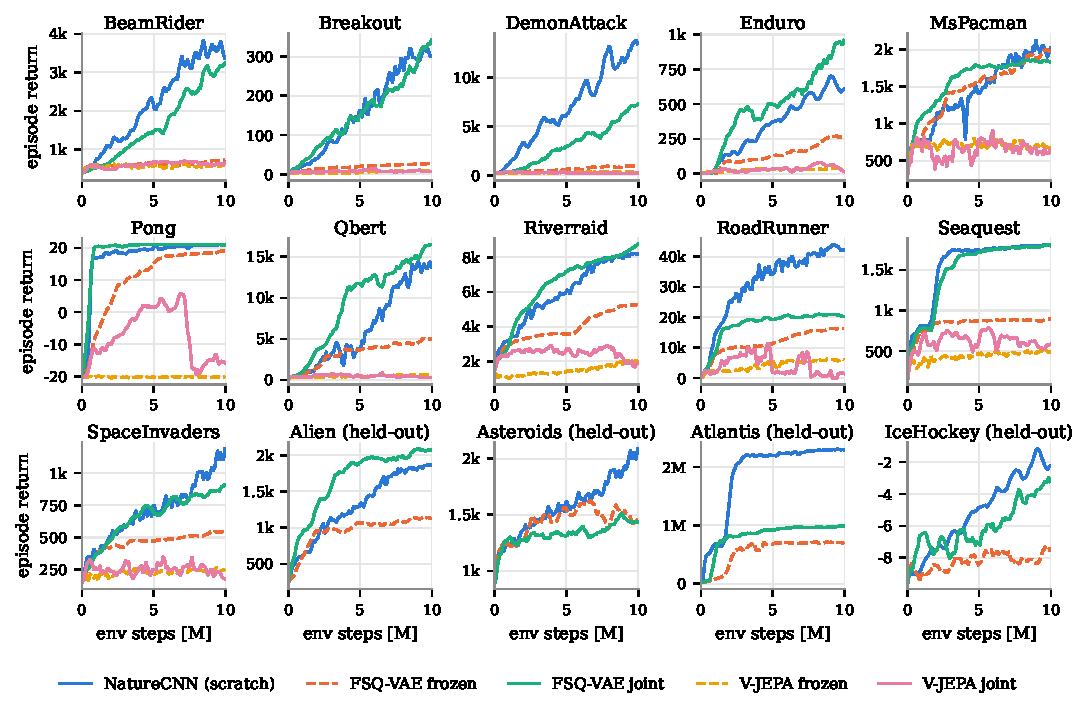
\includegraphics[width=\textwidth]{figures/learning_curves.pdf}\\[0.2em]
  {\footnotesize Solid: trained or fine-tuned encoders; dashed: frozen encoders}
\end{frame}

\begin{frame}{Results: Sample Efficiency}
  \begin{itemize}\setlength\itemsep{0.6em}
    \item I measured how many steps each agent needs to reach 50\% and 80\% of NatureCNN's
          final return
    \item At the 80\% level, \textbf{FSQ fine-tuned was faster} on Enduro, MsPacman, Qbert
          and Riverraid
      \begin{itemize}
        \item 1.4 to 2.6\,M steps earlier (19--39\% fewer steps)
      \end{itemize}
    \item At the 50\% level it was faster on 5 of 11 games
    \item NatureCNN was faster at both levels on the other six games; on MsPacman the FSQ agent
          learned faster but ended lower
  \end{itemize}
\end{frame}

\begin{frame}{Results: Can the V-JEPA Features Be Fixed?}
  \begin{itemize}\setlength\itemsep{0.55em}
    \item My first guess: the 9\,216-dimensional feature is too big for PPO
    \item So I repeated all 22 seen-game runs with the tokens averaged into a \textbf{256-dim}
          feature (these runs also used separate actor and critic encoders)
    \item And the frozen runs once more with a $5\times$ larger \textbf{entropy bonus}
  \end{itemize}
  \vspace{0.3em}
  \centering
  {\small
  \begin{tabular}{@{}llcc@{}}
    \toprule
    Feature & Mode & Median HNS & Critic expl.\ var. \\
    \midrule
    9\,216 (flat) & frozen & 0.045 & 0.73 \\
    256 (pooled) & frozen & 0.021 & 0.53 \\
    256 (pooled) & fine-tuned & 0.007 & $-0.27$ \\
    256, entropy 0.05 & frozen & 0.015 & 0.03 \\
    \bottomrule
  \end{tabular}}
  \vspace{0.5em}
  \begin{itemize}\small
    \item Neither change helped, so the size of the feature was probably not the problem, but
          the information in it
  \end{itemize}
\end{frame}

\begin{frame}{Results: World-Model Diagnostics}
  \begin{columns}[T]
    \begin{column}{0.57\textwidth}
      \begin{itemize}\small\setlength\itemsep{0.35em}
        \item Next states share 3 of 4 frames, so \textbf{copying} the current latent already
              looks good. I compared against that, an untrained model and \textbf{wrong actions}
        \item \textbf{No collapse:} effective rank 52.5 vs.\ 2.5 untrained
        \item \textbf{It learned dynamics:} better than copying, gap grows from $+0.013$
              (1 step) to $+0.046$ (5 steps)
        \item \textbf{But the action barely matters:} a wrong action changes the prediction by
              only 0.006
        \item The game token gets $1.8\times$ uniform attention, but the encoder already
              recognises the game from the pixels
        \item On held-out games it is worse than copying
      \end{itemize}
    \end{column}
    \begin{column}{0.43\textwidth}
      \centering
      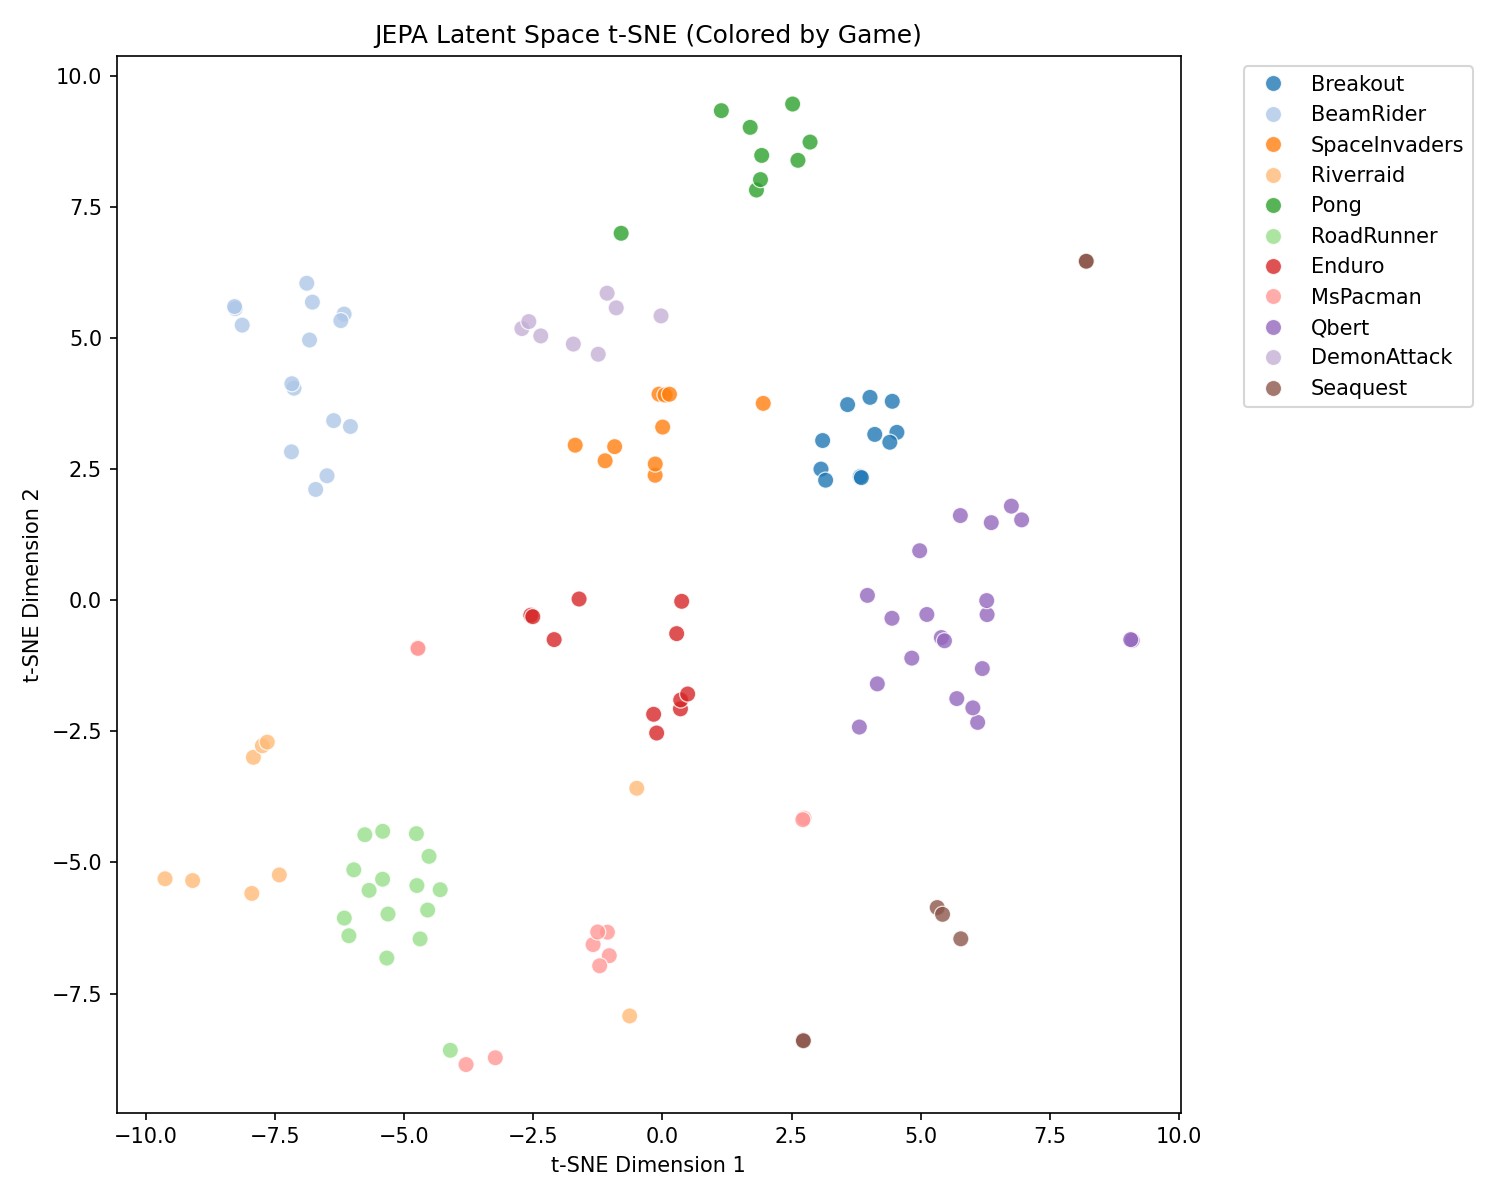
\includegraphics[width=\textwidth]{figures/jepa_tsne_by_game.png}\\[0.2em]
      {\scriptsize t-SNE of V-JEPA latents: they group by game}
    \end{column}
  \end{columns}
\end{frame}

\begin{frame}{Results: Why the V-JEPA Failed with PPO}
  \begin{columns}[T]
    \begin{column}{0.46\textwidth}
      \centering
      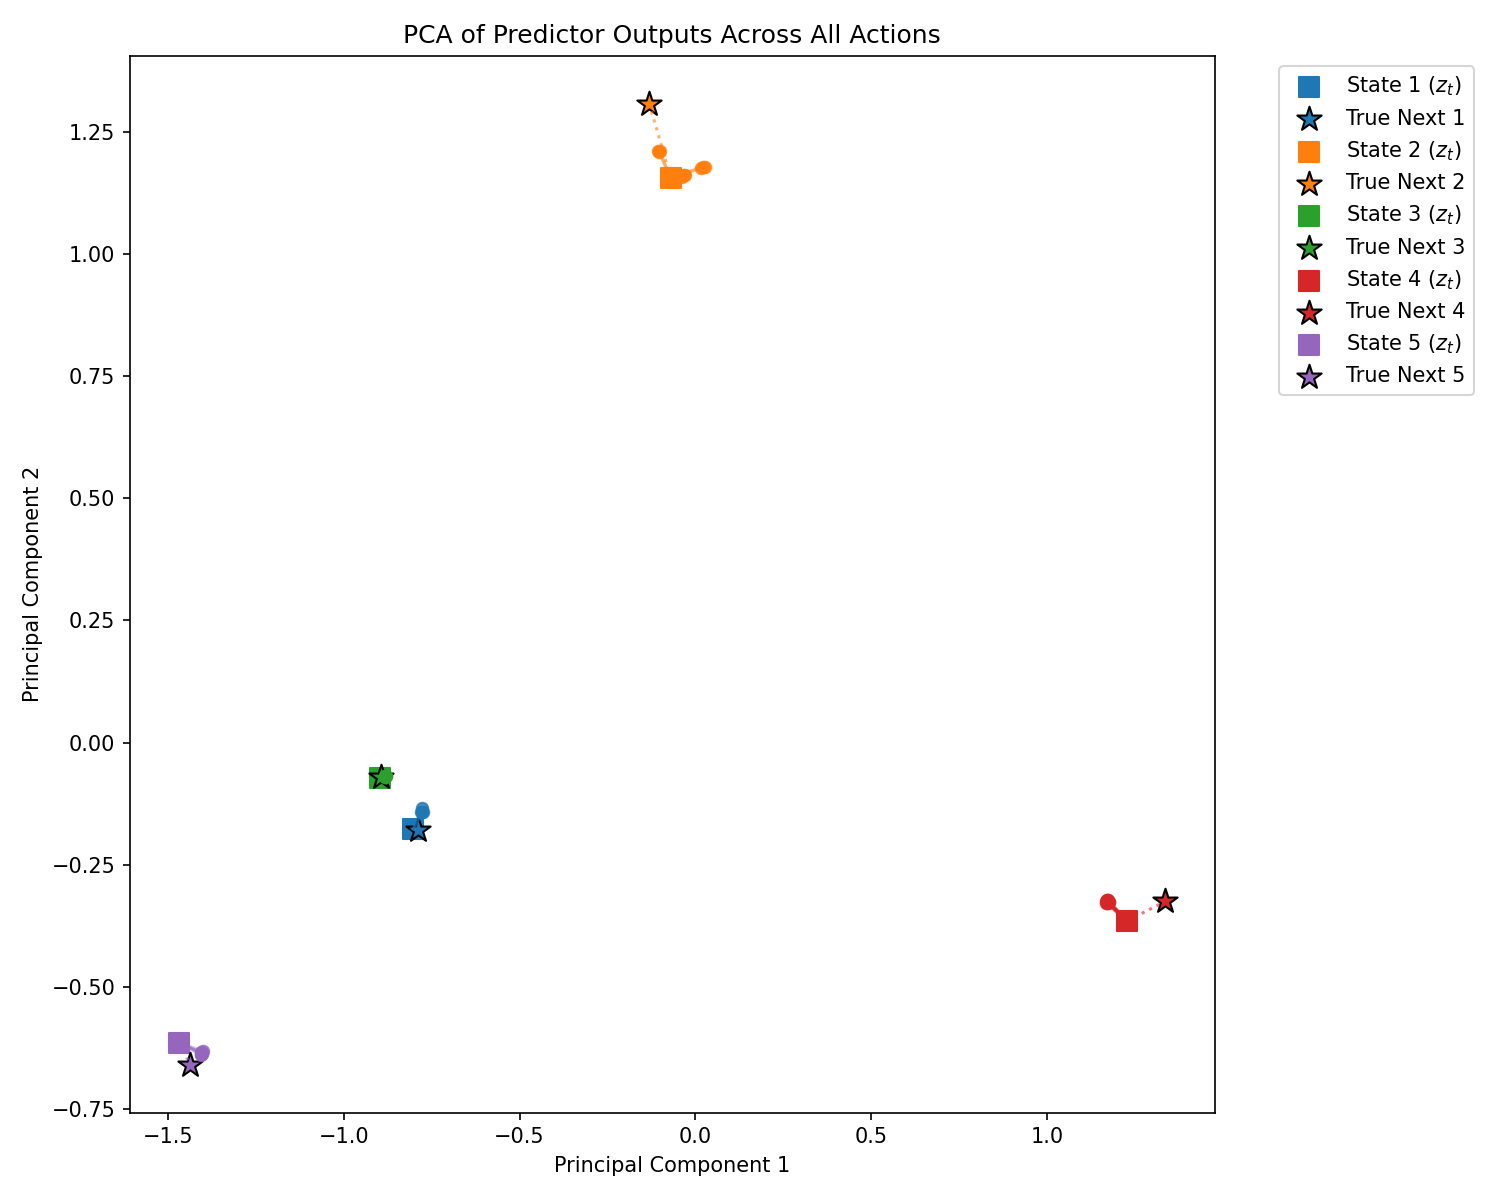
\includegraphics[width=\textwidth]{figures/pca_action_sensitivity.png}\\[0.2em]
      {\scriptsize The predictions for all actions (dots) land almost on the same spot}
    \end{column}
    \begin{column}{0.54\textwidth}
      \footnotesize
      \textbf{What I measured}
      \begin{itemize}\setlength\itemsep{0.1em}
        \item Predictor mostly ignores the action
        \item Latents barely change per step (cos.\ 0.974)
        \item Latent space is sorted by game
        \item Worse on held-out games
      \end{itemize}
      \vspace{0.3em}
      \textbf{What I think it means}
      \begin{itemize}\setlength\itemsep{0.1em}
        \item JEPA can ignore details with little effect on the latent error, like a small
              ball
        \item $14\times14$ patches are coarse for small objects
        \item Expert data shows few other actions
        \item The critic could read how good a state is, but the policy could not find the
              right action
      \end{itemize}
    \end{column}
  \end{columns}
\end{frame}

% =================================================================
\section{Conclusion}

\begin{frame}{Conclusion}
  \begin{itemize}\setlength\itemsep{0.55em}
    \item \textbf{RQ1:} the FSQ-VAE gave the most useful features when fine-tuned (beat Std-VAE on every game,
          Res-VQ on all but one)
    \item \textbf{RQ2:} fine-tuning worked much better than freezing
      \begin{itemize}
        \item FSQ fine-tuned vs.\ NatureCNN: higher median HNS (1.07 vs.\ 0.74) and faster
              learning on 4 games, but a better final score on only 4 of 11
      \end{itemize}
    \item \textbf{RQ3:} no overall gain on unseen games (FSQ better only on Alien, NatureCNN
          ahead on the other 3)
    \item \textbf{RQ4:} freezing the V-JEPA made PPO about 25\% faster (854 vs.\ 677 steps/s),
          but still slower than NatureCNN (976); the FSQ decoder shows what the features contain
    \item The V-JEPA learned how games usually evolve, but hardly what the agent's actions change
    \item \textbf{My answer:} a shared encoder is a useful starting point, but it cannot yet
          replace the NatureCNN when frozen
  \end{itemize}
\end{frame}

\begin{frame}{Limitations and Future Work}
  \begin{itemize}\setlength\itemsep{0.55em}
    \item \textbf{Limitations:} one seed per run, PPO not re-tuned for the pre-trained encoders
    \item \textbf{Future work:}
      \begin{itemize}\setlength\itemsep{0.3em}
        \item Repeat the main comparison with 3 seeds
        \item V-JEPA with smaller patches and a loss where the action matters more
              (multi-step prediction, reward head)
        \item Check the features first by predicting object positions, before running PPO
        \item Use the FSQ grid inside a world model, and pre-train on more games
      \end{itemize}
  \end{itemize}
\end{frame}

\begin{frame}
  \vfill
  \centering
  {\Huge\bfseries Thank You!}
  \vfill
\end{frame}

\end{document}
